\subsubsection{Entity-Relationship-Diagramm}
\begin{figure} [H]
    \centering
    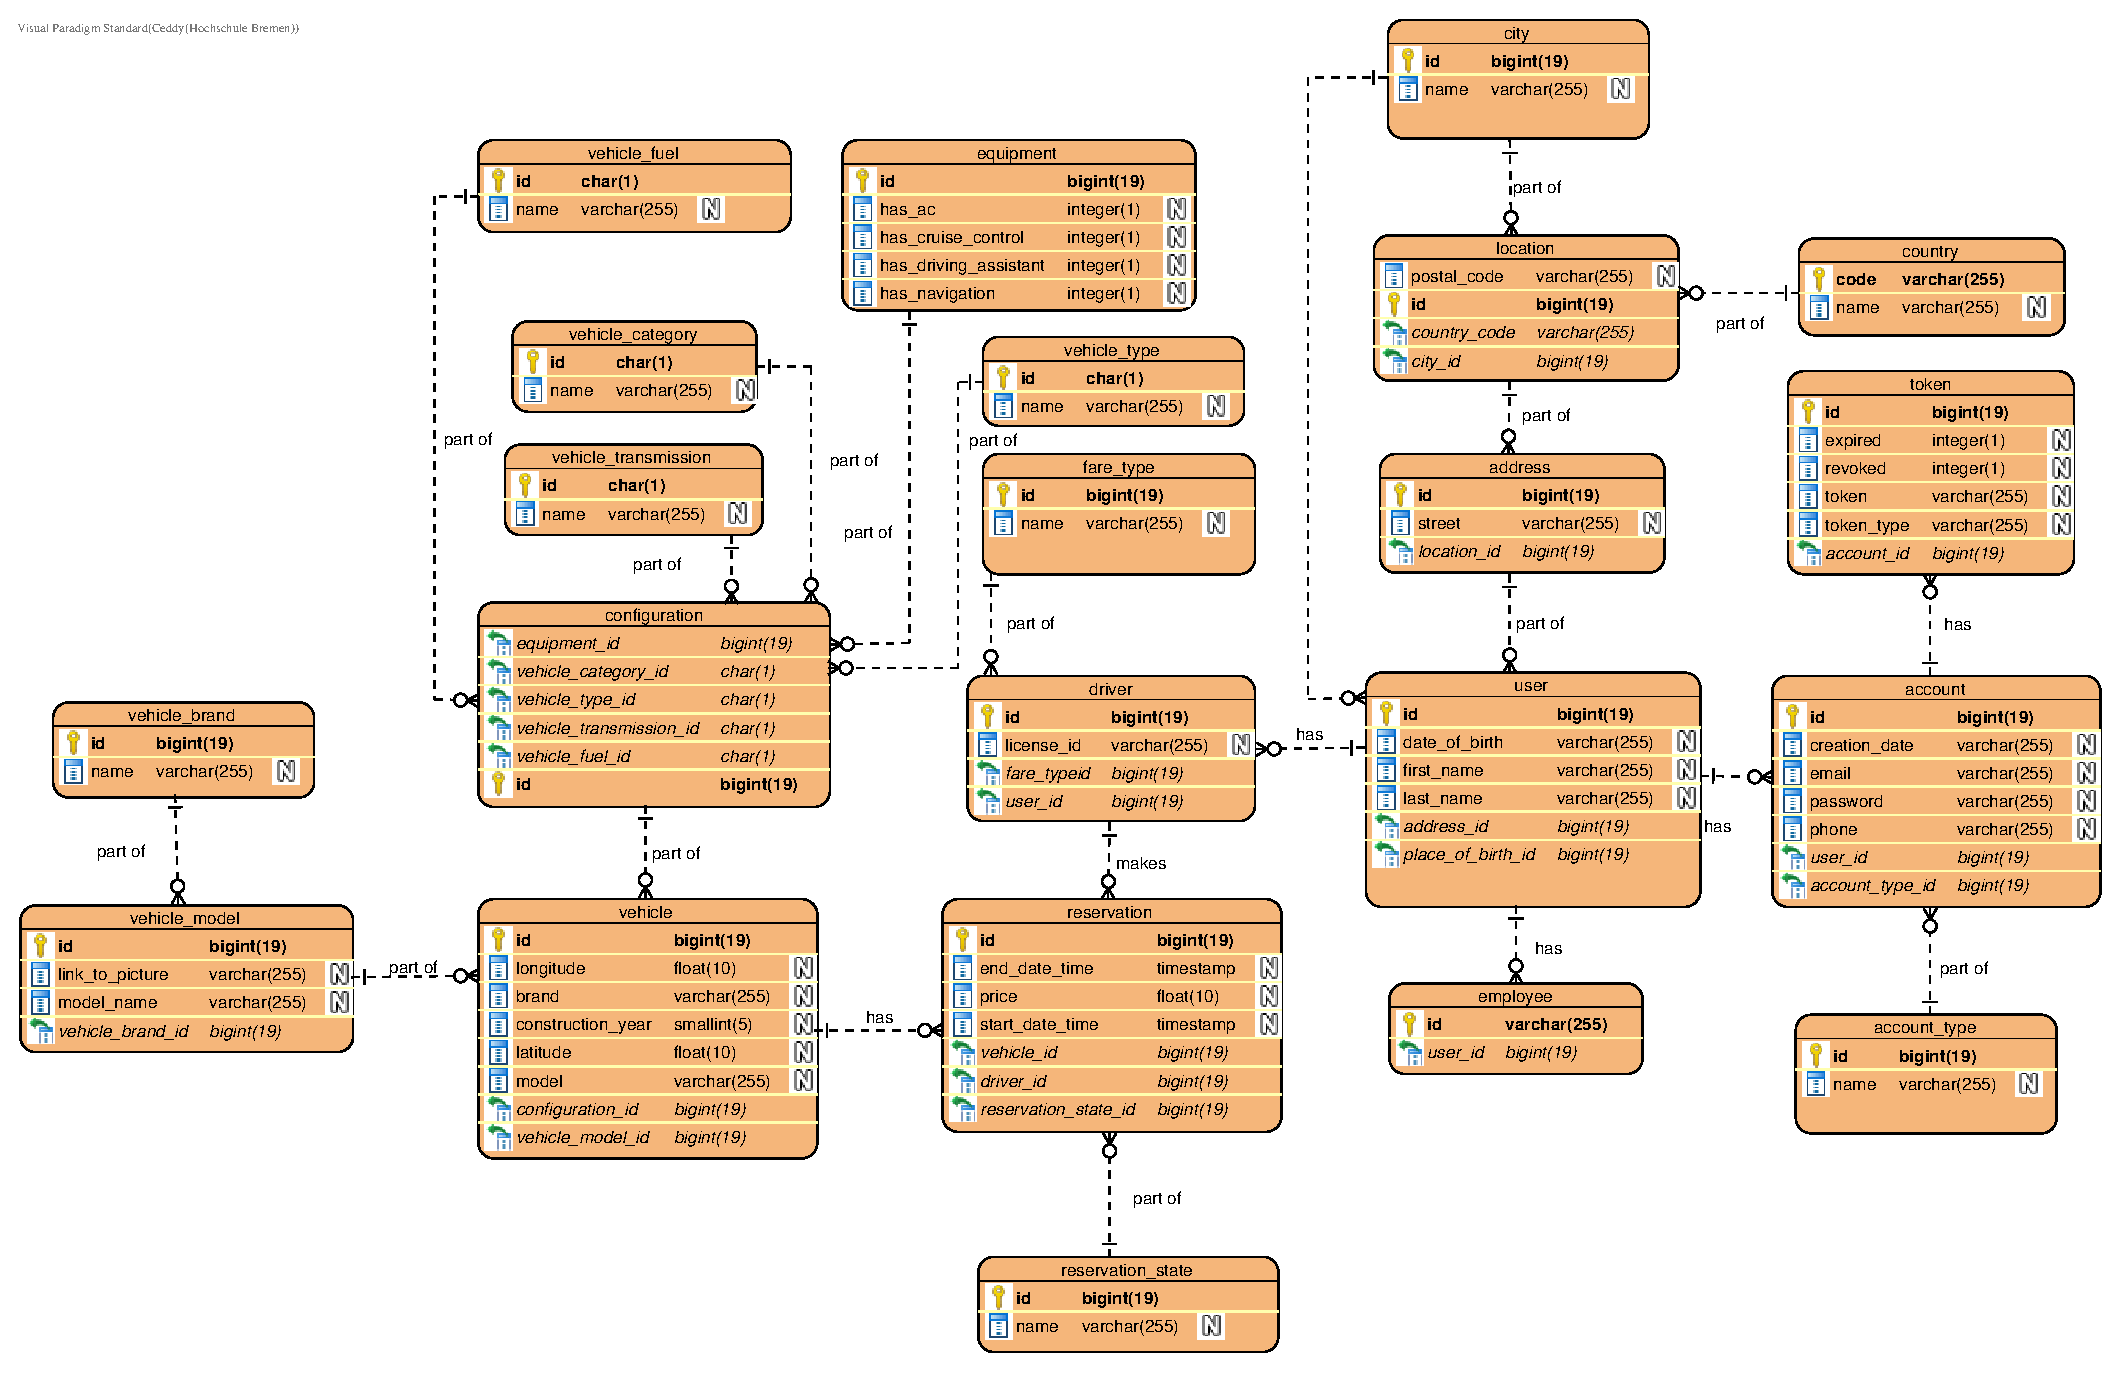
\includegraphics[width=1\textwidth]{pictures/Fastlane-ERD}
    \caption{Entity-Relationship-Diagramm}
    \label{fig:ERD}
\end{figure}

\bigskip

Das ER-Diagramm stellt die Entitäten und deren Relationen in der Datenbank des Systems dar.
Sowohl ein \enquote{Employee} als auch ein \enquote{Driver} können auf dieselbe natürliche Person verweisen.
Dies ermöglicht es, dass eine Person sowohl als Angestellter als auch als Fahrer agieren kann, je nach den Anforderungen und Rollen in diesem System.
Durch diese flexible Gestaltung kann gewährleistet werden, dass die Benutzer verschiedene Rollen und Funktionen zugewiesen können, ohne dass separate Benutzerinstanzen erstellt werden müssen.
Außerdem befindet sich die Datenbank in der dritten Normalform, was eine strukturierte und optimierte Speicherung der Daten gewährleistet.
Durch die Verwendung zentraler Entitäten und die Vermeidung unnötiger Dubletten können Änderungen effizient an einer einzigen Stelle vorgenommen werden, was die Wartung und Verwaltung erleichtert und potenzielle Inkonsistenzen minimiert.

\bigskip

\subsubsection{Deployment-Diagramm}

\begin{figure} [H]
    \centering
    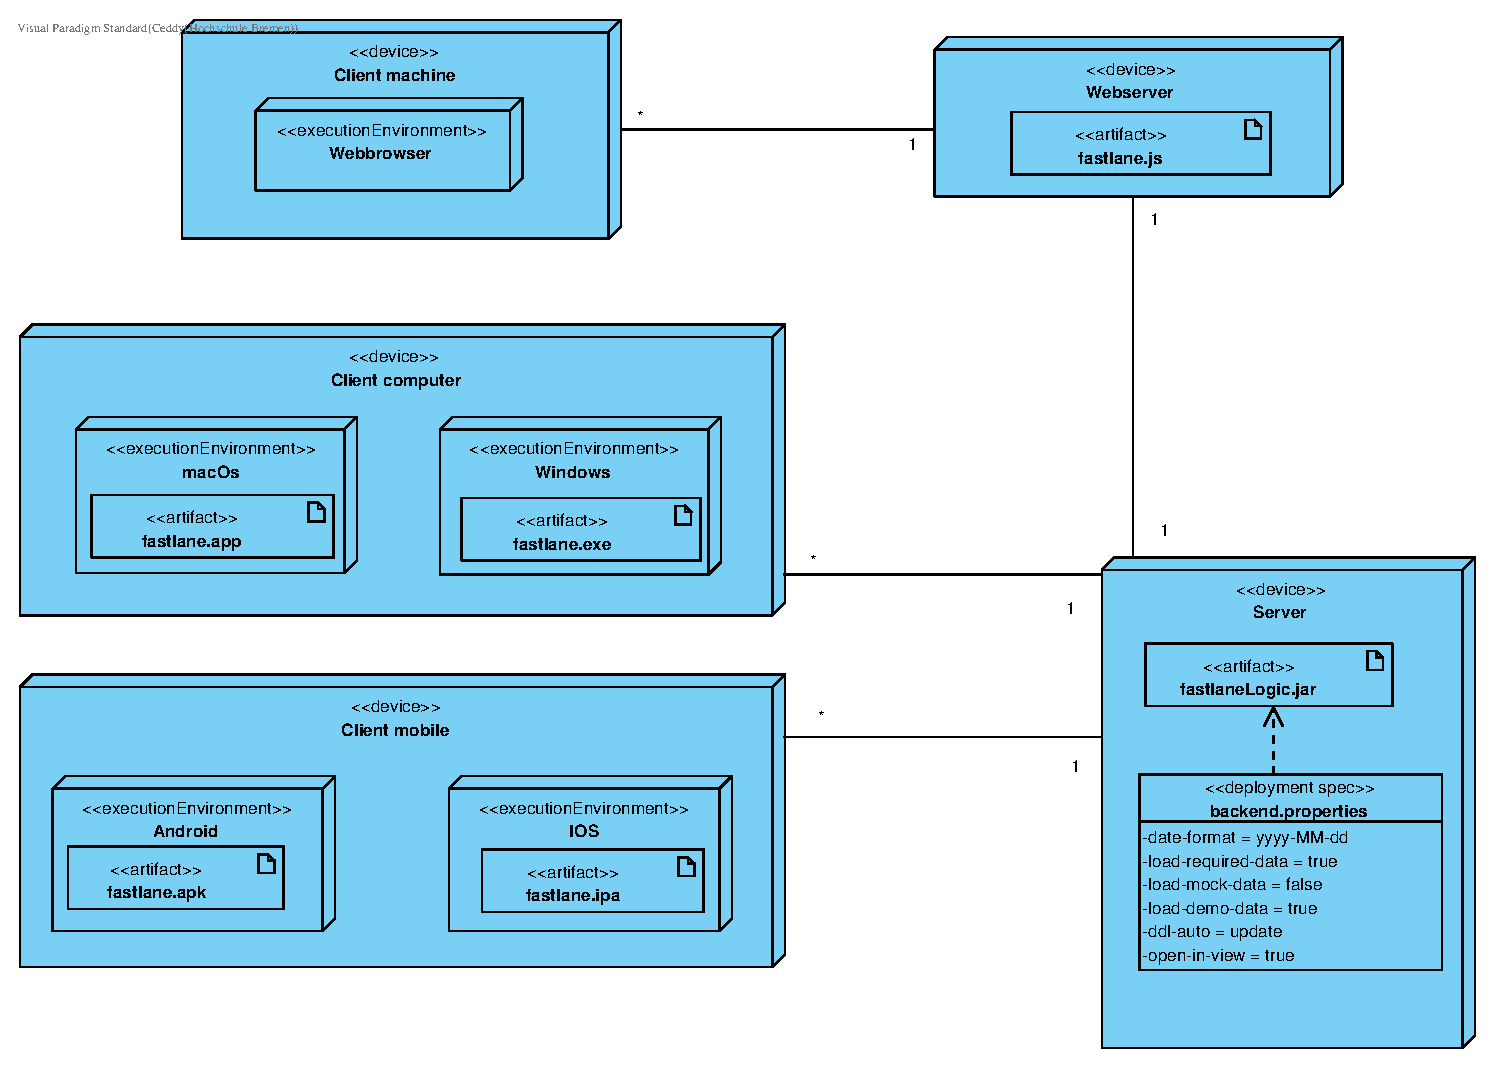
\includegraphics[width=1\textwidth]{pictures/Fastlane_Deployment_Diagram}
    \caption{Deployment-Diagramm}
    \label{fig:Deployment-Diagram}
\end{figure}

\bigskip


Das folgende Diagramm zeigt die Verteilung des Systems auf die verschiedenen Geräte und Ausführungsumgebungen.
Die Flexibilität von Flutter ermöglicht es, die Frontend-Anwendungen in verschiedenen Ausführungsumgebungen auszuführen, was eine entsprechende Verteilung erforderlich macht.
Die Backend-Anwendung wird auf einem dedizierten Server ausgeführt und stellt die Kernfunktionalität und Datenverarbeitung bereit.
Um die Daten für den Webbrowser auf beliebigen Geräten bereitzustellen, wird ein Webserver verwendet, der die Daten per HTTPS liefert.
In diesem Deployment-Diagramm wurde der Webbrowser auf einem Client-Device platziert, um die Ausführungsumgebung nicht doppelt auf dem Client-Computer und dem Client-Mobilgerät darstellen zu müssen.
Die ausführbaren Dateien, die das Frontend enthalten, werden in den Ausführungsumgebungen der jeweiligen Geräte ausgeführt.
Ein beispielhaftes Szenario zeigt die Ausführung der fastlane.apk auf einem Android-Gerät, das in der entsprechenden Umgebung auf einem Client-Mobilgerät läuft.
Durch diese Verteilung der Komponenten auf die Geräte und Ausführungsumgebungen kann die Software plattformübergreifend genutzt werden, wobei jedes Gerät die spezifischen Anforderungen der jeweiligen Ausführungsumgebung erfüllen muss.

\bigskip

\subsubsection{Sequenz-Diagramm}
\begin{figure}[H]
    \centering
    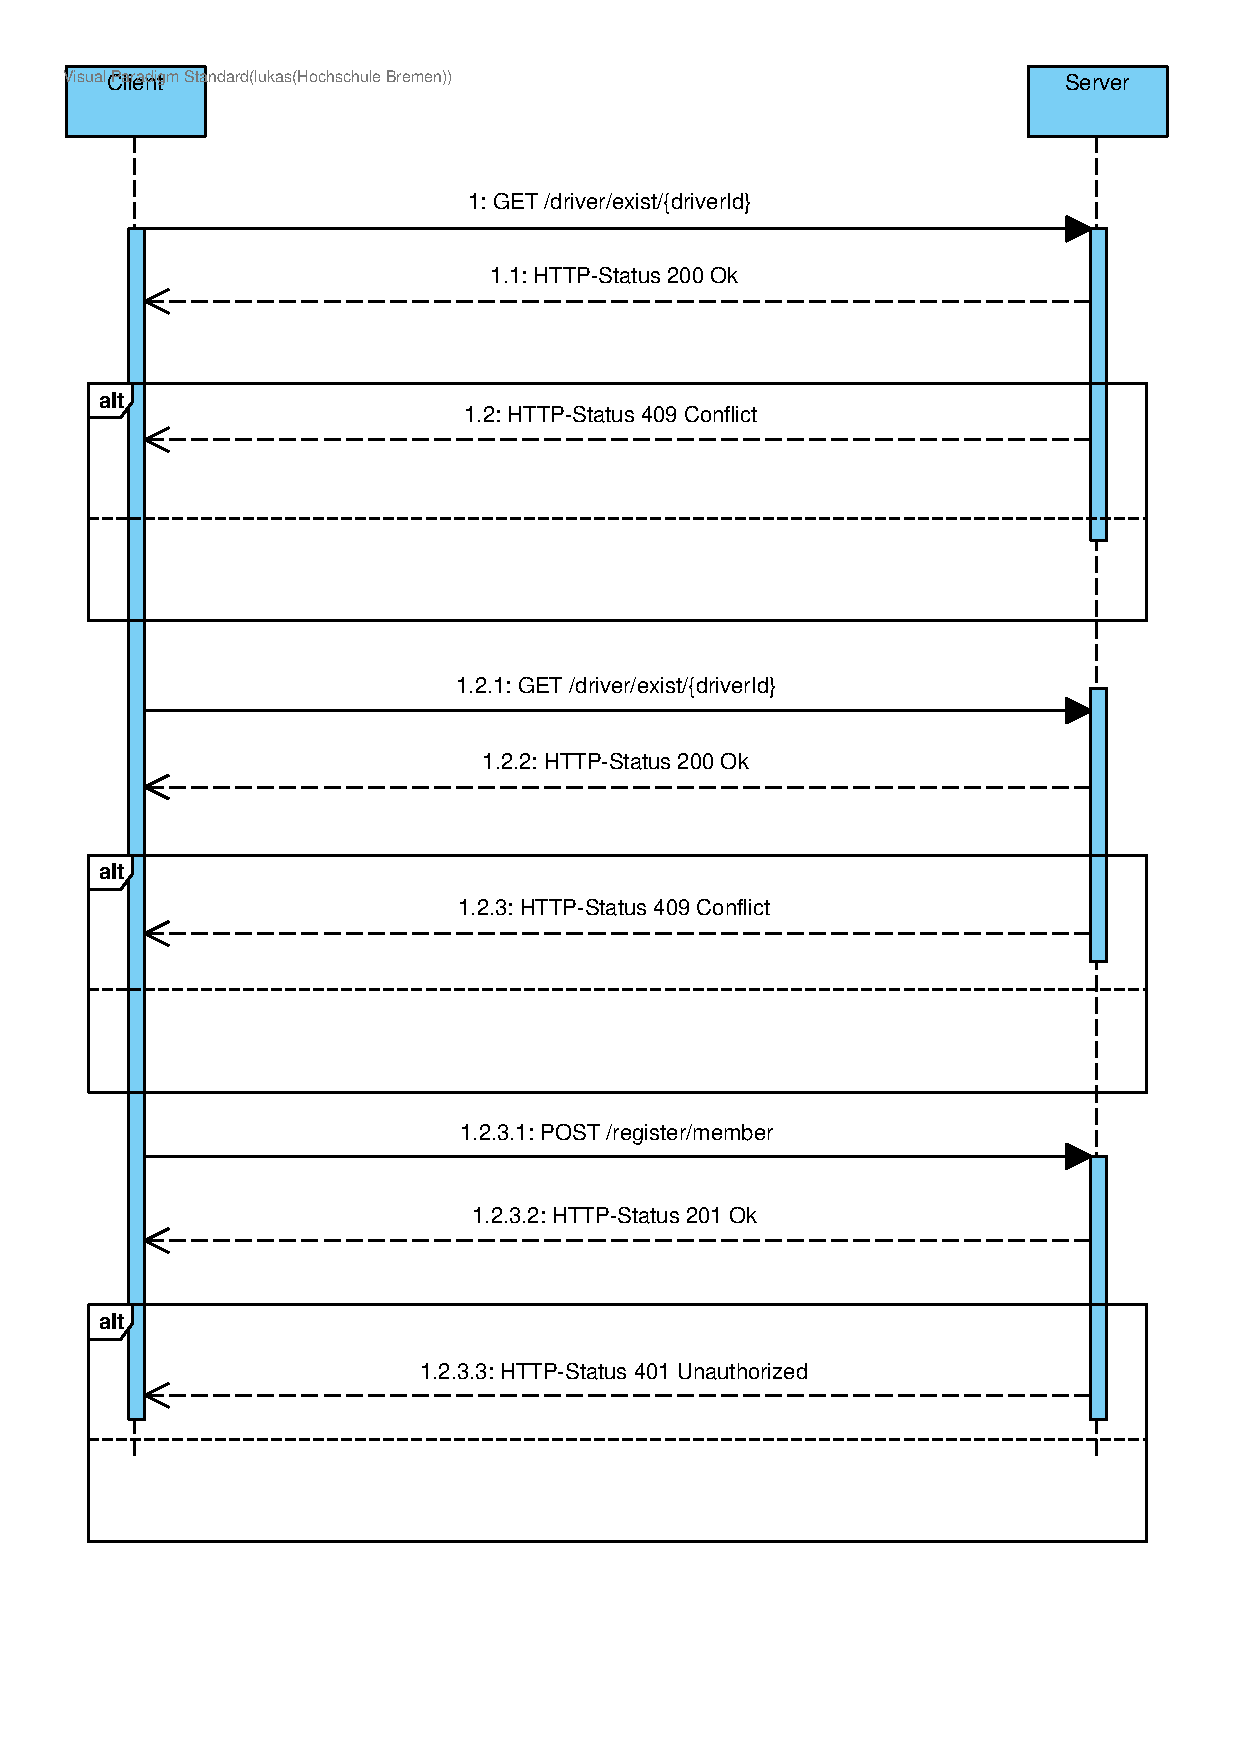
\includegraphics[width = 0.87\textwidth]{pictures/fastlane_sequenz_diagramm}
    \caption{Sequenzdiagramm}
    \label{fig:sequenzdiagramm}
\end{figure}

Das abgebildete Sequenzdiagramm stellt den Vorgang des Registrierens dar.
Dabei ist zu beachten, dass die Requests an die entsprechende Serveradresse gesendet werden.
Somit würde beispielsweise ein vollständiger Request an die localhost Adresse, über den Port 8080 folgendermaßen
aussehen: http://localhost:8080/driver/exist/licenseId.
Zu Beginn der Registrierung muss der Nutzer seine Führerschein Id eingeben.
Daher wird ein HTTP-Request an das Backend an den Endpunkt \enquote{/driver/exist/licenseId} gesendet.
Existiert die Führerschein Id noch nicht, so wird der Status Code 200 Ok zurückgesendet.
Ist die Id allerdings schon im System vorhanden, wir der Status Code 409 Conflict
zurückgesendet. \medskip

Zu einem späteren Zeitpunkt der Registrierung wird vom Benutzer eine E-Mail eingegeben.
Dabei läuft der gleiche Prozess erneut ab.
Es wird ein HTTP-Request an den Endpunkt \enquote{account/exist/email} gesendet.
Wenn die E-Mail bereits im System existiert, wird der Status Code 409 Conflict zurückgesendet.
Existiert sie allerdings noch nicht, wird der Status Code 200 Ok gesendet. \medskip

Sobald der Nutzer mit der Eingabe seiner Daten fertig ist, wird ein Post Request an den
Endpunkt \enquote{/register/member} gesendet.
Dabei werden im Body des Requests alle eingegebenen Daten mitgegeben.
Sofern die Registrierung im Backend erfolgreich verläuft, wird der Status Code 201 Created gesendet.
Tritt jedoch ein Fehler auf, wird der Status Code 401 Unauthorized zurückgesendet. \medskip

Dieses Diagramm stellt nur die Registrierung dar, allerdings laufen die meisten Prozesse nach dem gleichen Prinzip
ab.
Sobald im Frontend ein Request gesendet wird, wird dieser im Backend verarbeitet und der Entsprechende Status Code
mit dem Passenden Body zurückgesendet.